\section{1174066 - D.Irga B. Naufal Fakhri}
\subsection{Teori}
\subsubsection{Kenapa file teks harus di lakukan tokenizer}
\hfill\break
Karena MTokenizer adalah proses membagi teks yang berupa kalimat, paragraf atau dokumen menjadi kata-kata atau bagian-bagian tertentu dalam kalimat tersebut. Contohnya kalimat "Tugas chapter 7", kalimat itu menjadi beberapa bagian yaitu "Tugas", "chapter", "7". Yang menjadi acuan yakni tanda baca dan spasi.
\begin{figure}[H]
\centering
	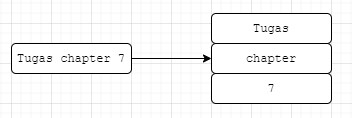
\includegraphics[width=4cm]{figures/1174066/7/1.jpg}
\caption{Teori 1}
\end{figure}

\subsubsection{konsep dasar K Fold Cross Validation pada dataset komentar Youtube pada kode listing 7.1.}
\hfill\break
Konsep sederhana dari K Fold Cross Validation ialah Pada code ini:
\lstinputlisting[firstline=12, lastline=13]{src/1174066/7/1.py}
terdapat kfold yang bertujuan untuk melakukan split data menjadi 5 bagian dari dataset komentar Youtube tersebut. Sehingga dari setiap data yang sudah dibagi tersebut akan menghasilkan presentase dari setiap bagiannya, untuk menghasilkan hasil akhir dengan presentase yang cukup baik.
\begin{figure}[H]
\centering
	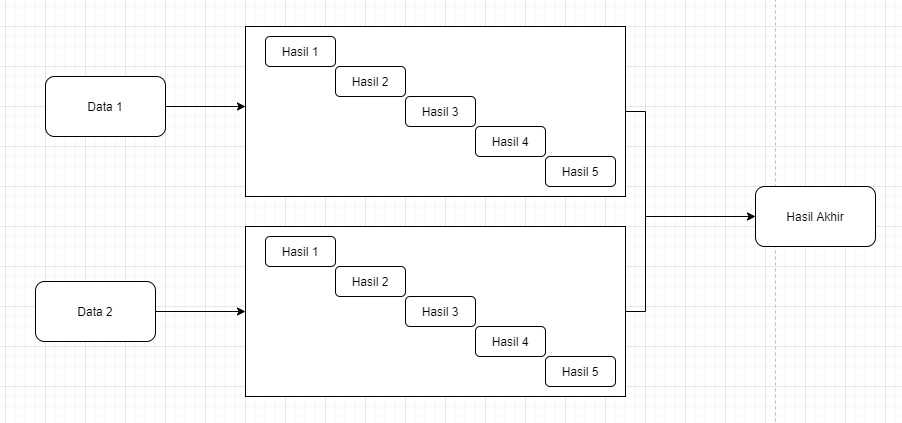
\includegraphics[width=4cm]{figures/1174066/7/2.jpg}
\caption{Teori 2}
\end{figure}

\subsubsection{Apa maksudnya kode program for train, test in splits}
\hfill\break
For train berfungsi untuk membagi data tersebut menjadi data training. Sedangkan test in splits berfungsi untuk menguji apakah dataset tersebut sudah dibagi menjadi beberapa bagian atau masih menumpuk.
\begin{figure}[H]
\centering
	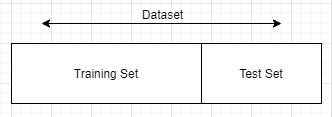
\includegraphics[width=4cm]{figures/1174066/7/3.jpg}
\caption{Teori 3}
\end{figure}

\subsubsection{Apa maksudnya kode program train content = d[’CONTENT’].iloc[train idx] dan test content = d[’CONTENT’].iloc[test idx]}
\hfill\break
Fungsi dalam kode tersebut berfungsi untuk mengambil data pada kolom atau index CONTENT yang merupakan bagian dari train\_idx dan test\_idx. Contoh sederhananya ketika data telah diubah menjadi data train dan data test maka kita dapat memilihnya untuk ditampilkan pada kolom yang di inginkan. 
\lstinputlisting[firstline=15, lastline=21]{src/1174066/7/1.py}
\begin{figure}[H]
\centering
	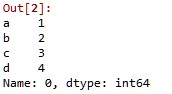
\includegraphics[width=4cm]{figures/1174066/7/4.jpg}
\caption{Teori 4}
\end{figure}

\subsubsection{Apa maksud dari fungsi tokenizer = Tokenizer(num words=2000) dan tokenizer.fit on texts(train content)}
\hfill\break
Fungsi tokenizer berfungsi untuk melakukan vektorisasi data kedalam bentuk token sebanyak 2000 kata. Dan selanjutnya akan melakukan fit tokenizer hanya untuk data training saja tidak dengan data testingnya.
\begin{figure}[H]
\centering
	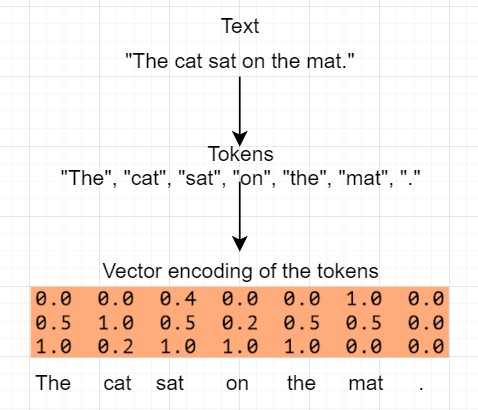
\includegraphics[width=4cm]{figures/1174066/7/5.jpg}
\caption{Teori 5}
\end{figure}

\subsubsection{Apa maksud dari fungsi d train inputs = tokenizer.texts to matrix(train content, mode=’tfidf ’) dan d test inputs = tokenizer.texts to matrix(test content, mode=’tfidf ’)}
\hfill\break
Maksud dari baris diatas ialah untuk memasukkan text ke sebuah matrix dengan mode tfidf dan menginputkan data testing untuk di terjemahkan ke sebuah matriks.
\begin{figure}[H]
\centering
	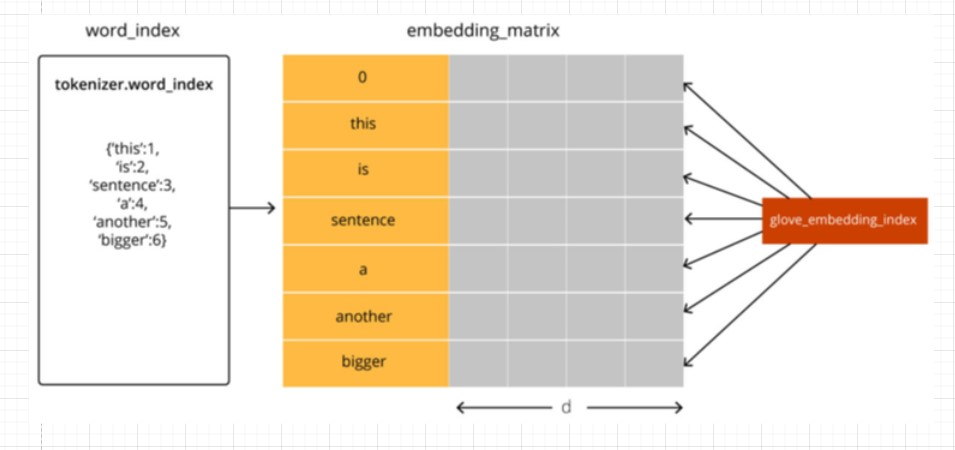
\includegraphics[width=4cm]{figures/1174066/7/6.jpg}
\caption{Teori 6}
\end{figure}

\subsubsection{Apa maksud dari fungsi d train inputs = d train inputs/np.amax(np.absolute(d train inputs)) dan d test inputs = d test inputs/np.amax(np.absolute(d test inputs))}
\hfill\break
Fungsi np.amax adalah nilai Maksimal. Jika sumbu tidak ada, hasilnya adalah nilai skalar. Jika sumbu diberikan, hasilnya adalah array dimensi a.ndim - 1.
\begin{figure}[H]
\centering
	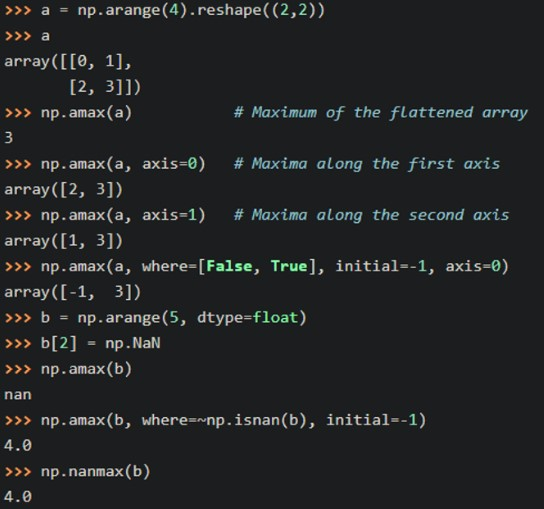
\includegraphics[width=4cm]{figures/1174066/7/7.jpg}
\caption{Teori 7}
\end{figure}

\subsubsection{Apa maksud fungsi dari d train outputs = np utils.to categorical(d[’CLASS’].iloc[train idx]) dan d test outputs = np utils.to categorical(d[’CLASS’].iloc[test idx]) dalam kode program}
\hfill\break
Fungsi dari baris kode tersebut ialah membuat train outputs dengan kategori dari class lalu dengan ketentuan iloc train idx. Kemudian membuat keluaran sebagai output.
\begin{figure}[H]
\centering
	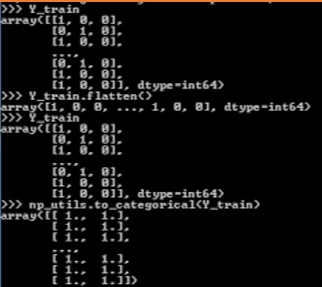
\includegraphics[width=4cm]{figures/1174066/7/8.jpg}
\caption{Teori 8}
\end{figure}

\subsubsection{Apa maksud dari fungsi di listing 7.2.}
\hfill\break
\lstinputlisting[firstline=26, lastline=31]{src/1174066/7/1.py}
Fungsi dari baris kode tersebut ialah model perlu mengetahui bentuk input apa yang harus diharapkan. Untuk alasan ini, lapisan pertama dalam model Sequential (dan hanya yang pertama, karena lapisan berikut dapat melakukan inferensi bentuk otomatis) perlu menerima informasi tentang bentuk inputnya.
\begin{figure}[H]
\centering
	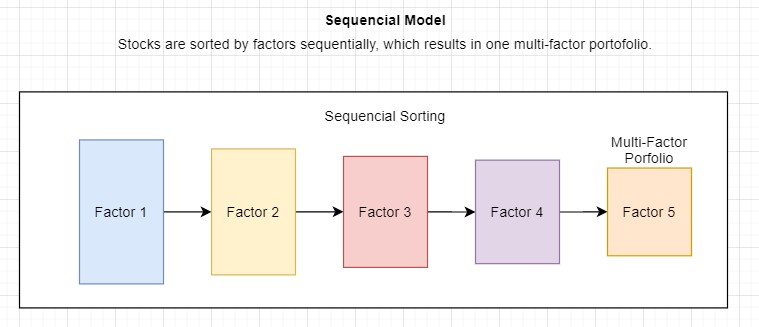
\includegraphics[width=4cm]{figures/1174066/7/9.jpg}
\caption{Teori 9}
\end{figure}

\subsubsection{Apa maksud dari fungsi di listing 7.3 dengan parameter tersebut}
\hfill\break
\lstinputlisting[firstline=34, lastline=35]{src/1174066/7/1.py}
Fungsi dari baris kode tersebut ialah bisa meneruskan nama fungsi loss yang ada, atau melewati fungsi simbolis TensorFlow yang mengembalikan skalar untuk setiap titik data dan mengambil dua argumen y\_true: True label. dan  y\_pred: Prediksi. Tujuan yang dioptimalkan sebenarnya adalah rata-rata dari array output di semua titik data.
\begin{figure}[H]
\centering
	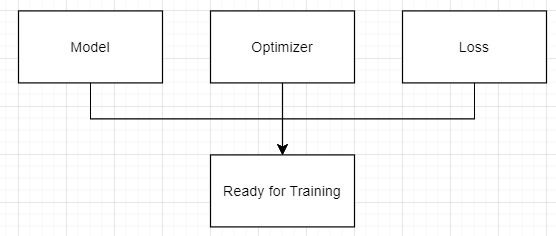
\includegraphics[width=4cm]{figures/1174066/7/10.jpg}
\caption{Teori 10}
\end{figure}

\subsubsection{Apa itu Deep Learning}
\hfill\break
Deep Learning adalah salah satu cabang dari ilmu machine learning yang terdiri dari algoritma pemodelan abstraksi tingkat tinggi pada data menggunakan sekumpulan fungsi transformasi non-linear yang ditata berlapis-lapis dan mendalam. Teknik dan algoritma dalam machine learning dapat digunakan baik untuk supervised learning dan unsupervised learning.

\subsubsection{Apa itu Deep Neural Network, dan apa bedanya dengan Deep Learning}
\hfill\break
Deep Neural Network adalah salah satu algoritma berbasis jaringan saraf tiruan yang memiliki dari 1 lapisan saraf tersembunyi yang dapat digunakan untuk pengambilan keputun. Perbedaannya dengan deep learning, yakni: Deep Neural Network dapat menentukan dan mencerna karakteristik tertentu di suatu rangkaian data, kapabilitas lebih kompleks untuk mempelajari, mencerna, dan mengklasifikasikan data, serta dibagi ke dalam berbagai lapisan dengan fungsi yang berbeda-beda.

\subsubsection{Jelaskan dengan ilustrasi gambar buatan sendiri(langkah per langkah) bagaimana perhitungan algoritma konvolusi dengan ukuran stride (NPM mod3+1) x (NPM mod3+1) yang terdapat max pooling.}	
\hfill\break
Konvolusi terdapat pada operasi pengolahan citra yang mengalikan sebuah citra dengan sebuah mask atau kernel, Stride adalah parameter yang berfungsi untuk menentukan pergeseran pada filter data pixel yang terjadi. untuk contoh penggunaannya:
\begin{figure}[H]
\centering
	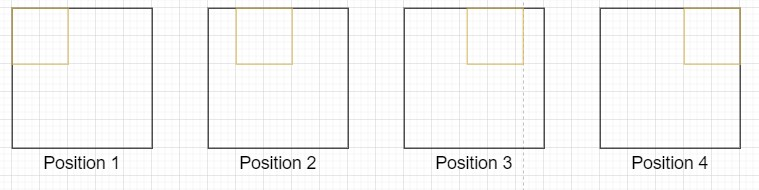
\includegraphics[width=4cm]{figures/1174066/7/11.jpg}
\caption{Teori 11}
\end{figure}



\subsection{Praktek}
\subsubsection{Nomor 1}
\hfill\break
\lstinputlisting[firstline=9, lastline=11]{src/1174066/7/2.py}
Hasil:
\begin{figure}[H]
\centering
	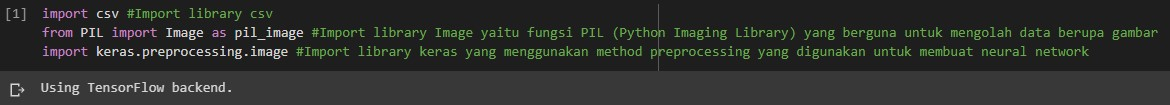
\includegraphics[width=4cm]{figures/1174066/7/no1.jpg}
	\caption{Hasil No 1}
\end{figure}

\subsubsection{Nomor 2}
\hfill\break
\lstinputlisting[firstline=14, lastline=27]{src/1174066/7/2.py}
Hasil:
\begin{figure}[H]
\centering
	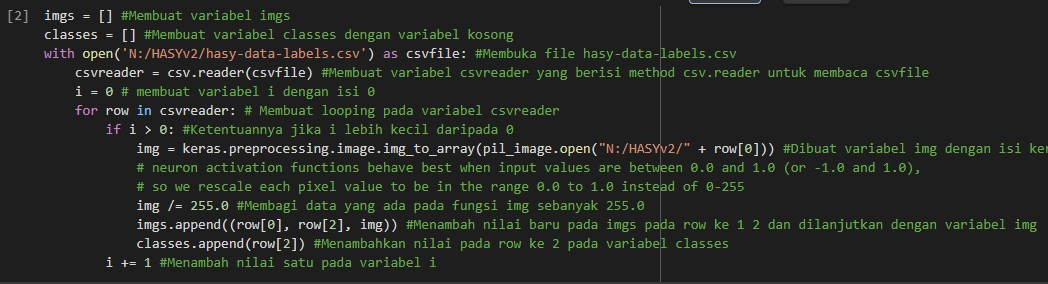
\includegraphics[width=4cm]{figures/1174066/7/no2.jpg}
	\caption{Hasil No 2}
\end{figure}

\subsubsection{Nomor 3}
\hfill\break
\lstinputlisting[firstline=30, lastline=34]{src/1174066/7/2.py}
Hasil:
\begin{figure}[H]
\centering
	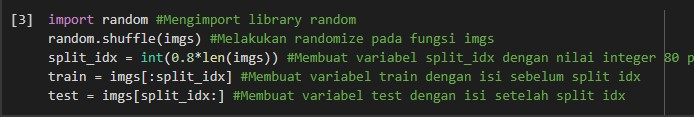
\includegraphics[width=4cm]{figures/1174066/7/no3.jpg}
	\caption{Hasil No 1}
\end{figure}

\subsubsection{Nomor 4}
\hfill\break
\lstinputlisting[firstline=37, lastline=41]{src/1174066/7/2.py}
Hasil:
\begin{figure}[H]
\centering
	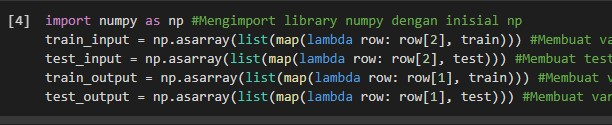
\includegraphics[width=4cm]{figures/1174066/7/no4.jpg}
	\caption{Hasil No 4}
\end{figure}

\subsubsection{Nomor 5}
\hfill\break
\lstinputlisting[firstline=44, lastline=45]{src/1174066/7/2.py}
Hasil:
\begin{figure}[H]
\centering
	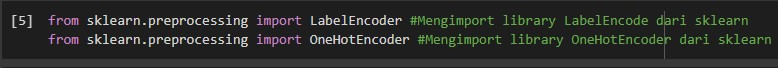
\includegraphics[width=4cm]{figures/1174066/7/no5.jpg}
	\caption{Hasil No 5}
\end{figure}

\subsubsection{Nomor 6}
\hfill\break
\lstinputlisting[firstline=48, lastline=49]{src/1174066/7/2.py}
Hasil:
\begin{figure}[H]
\centering
	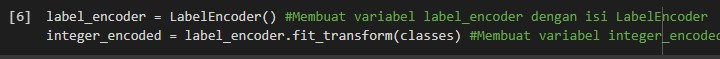
\includegraphics[width=4cm]{figures/1174066/7/no6.jpg}
	\caption{Hasil No 6}
\end{figure}

\subsubsection{Nomor 7}
\hfill\break
\lstinputlisting[firstline=52, lastline=54]{src/1174066/7/2.py}
Hasil:
\begin{figure}[H]
\centering
	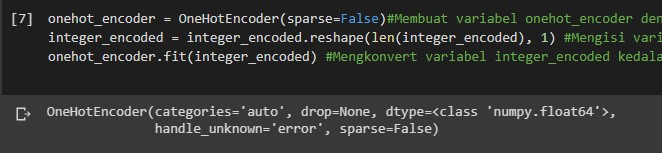
\includegraphics[width=4cm]{figures/1174066/7/no7.jpg}
	\caption{Hasil No 7}
\end{figure}

\subsubsection{Nomor 8}
\hfill\break
\lstinputlisting[firstline=57, lastline=62]{src/1174066/7/2.py}
Hasil:
\begin{figure}[H]
\centering
	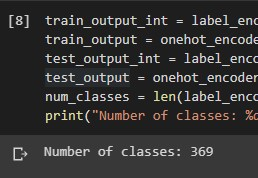
\includegraphics[width=4cm]{figures/1174066/7/no8.jpg}
	\caption{Hasil No 8}
\end{figure}

\subsubsection{Nomor 9}
\hfill\break
\lstinputlisting[firstline=65, lastline=67]{src/1174066/7/2.py}
Hasil:
\begin{figure}[H]
\centering
	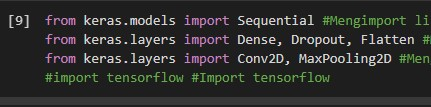
\includegraphics[width=4cm]{figures/1174066/7/no9.jpg}
	\caption{Hasil No 9}
\end{figure}

\subsubsection{Nomor 10}
\hfill\break
\lstinputlisting[firstline=71, lastline=83]{src/1174066/7/2.py}
Hasil:
\begin{figure}[H]
\centering
	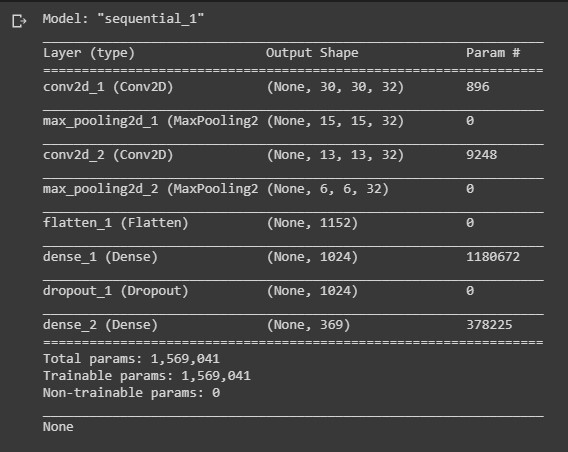
\includegraphics[width=4cm]{figures/1174066/7/no10.jpg}
	\caption{Hasil No 10}
\end{figure}

\subsubsection{Nomor 11}
\hfill\break
\lstinputlisting[firstline=86, lastline=87]{src/1174066/7/2.py}
Hasil:
\begin{figure}[H]
\centering
	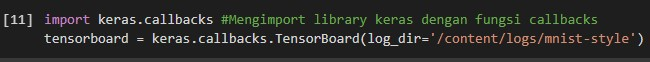
\includegraphics[width=4cm]{figures/1174066/7/no11.jpg}
	\caption{Hasil No 11}
\end{figure}

\subsubsection{Nomor 12}
\hfill\break
\lstinputlisting[firstline=90, lastline=99]{src/1174066/7/2.py}
Hasil:
\begin{figure}[H]
\centering
	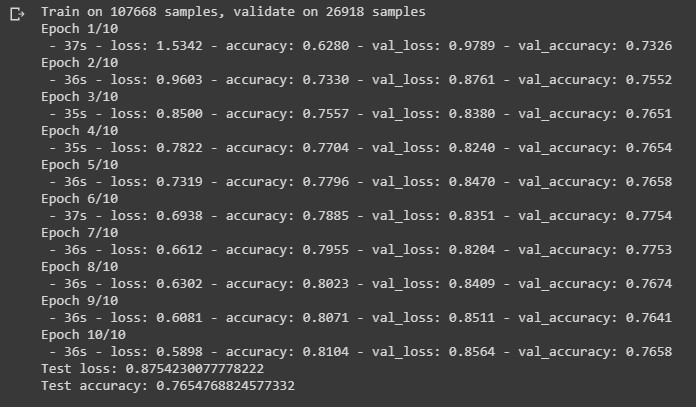
\includegraphics[width=4cm]{figures/1174066/7/no12.jpg}
	\caption{Hasil No 12}
\end{figure}

\subsubsection{Nomor 13}
\hfill\break
\lstinputlisting[firstline=102, lastline=130]{src/1174066/7/2.py}
Hasil:
\begin{figure}[H]
\centering
	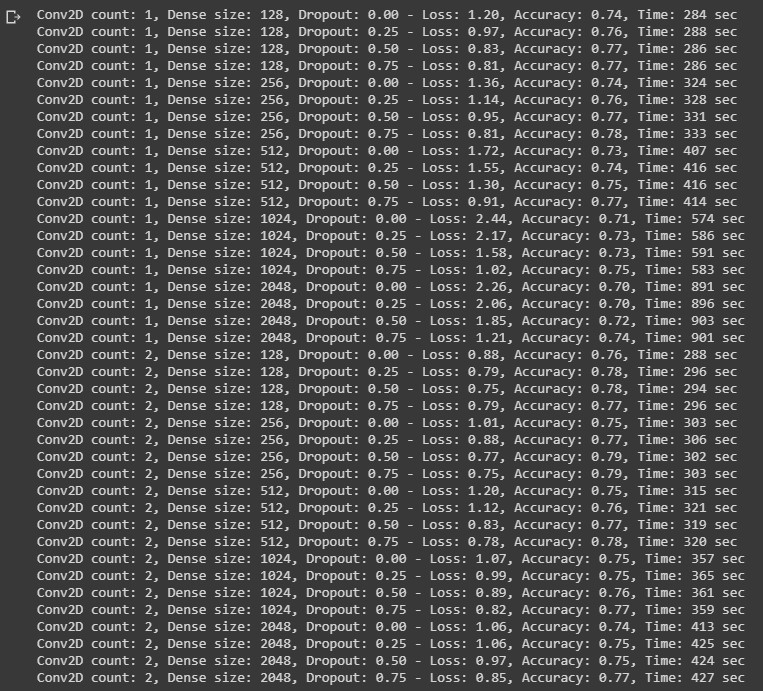
\includegraphics[width=4cm]{figures/1174066/7/no13.jpg}
	\caption{Hasil No 13}
\end{figure}

\subsubsection{Nomor 14}
\hfill\break
\lstinputlisting[firstline=133, lastline=143]{src/1174066/7/2.py}
Hasil:
\begin{figure}[H]
\centering
	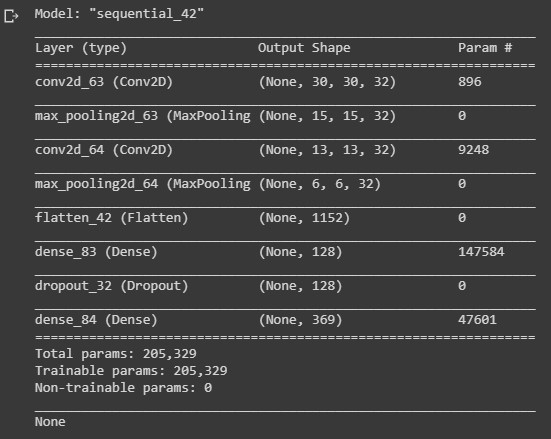
\includegraphics[width=4cm]{figures/1174066/7/no14.jpg}
	\caption{Hasil No 14}
\end{figure}

\subsubsection{Nomor 15}
\hfill\break
\lstinputlisting[firstline=146, lastline=148]{src/1174066/7/2.py}
Hasil:
\begin{figure}[H]
\centering
	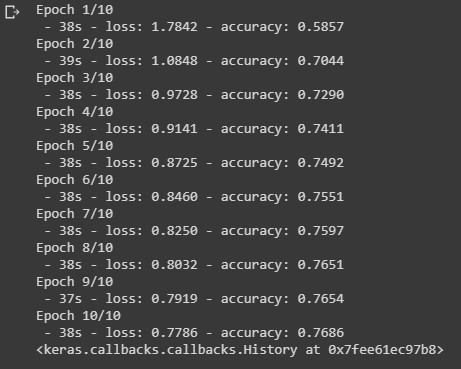
\includegraphics[width=4cm]{figures/1174066/7/no15.jpg}
	\caption{Hasil No 15}
\end{figure}

\subsubsection{Nomor 16}
\hfill\break
\lstinputlisting[firstline=151, lastline=151]{src/1174066/7/2.py}
Hasil:
\begin{figure}[H]
\centering
	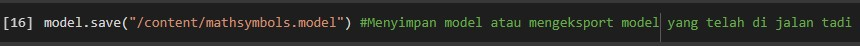
\includegraphics[width=4cm]{figures/1174066/7/no16.jpg}
	\caption{Hasil No 16}
\end{figure}

\subsubsection{Nomor 17}
\hfill\break
\lstinputlisting[firstline=154, lastline=154]{src/1174066/7/2.py}
Hasil:
\begin{figure}[H]
\centering
	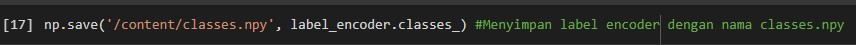
\includegraphics[width=4cm]{figures/1174066/7/no17.jpg}
	\caption{Hasil No 17}
\end{figure}

\subsubsection{Nomor 18}
\hfill\break
\lstinputlisting[firstline=158, lastline=160]{src/1174066/7/2.py}
Hasil:
\begin{figure}[H]
\centering
	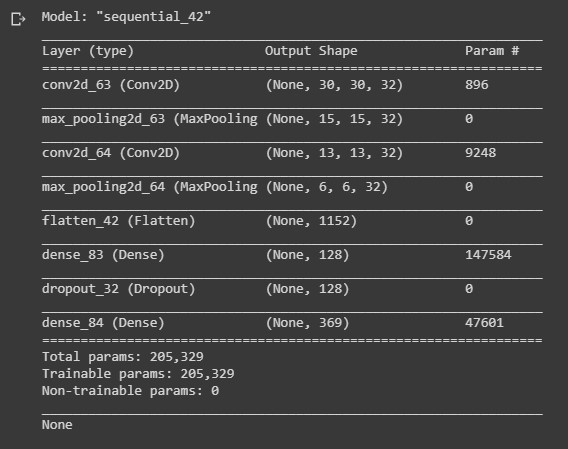
\includegraphics[width=4cm]{figures/1174066/7/no18.jpg}
	\caption{Hasil No 18}
\end{figure}

\subsubsection{Nomor 19}
\hfill\break
\lstinputlisting[firstline=163, lastline=174]{src/1174066/7/2.py}
Hasil:
\begin{figure}[H]
\centering
	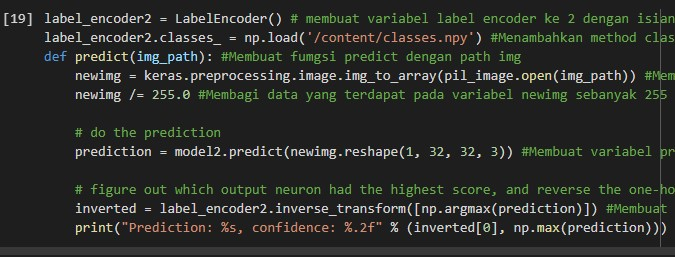
\includegraphics[width=4cm]{figures/1174066/7/no19.jpg}
	\caption{Hasil No 19}
\end{figure}

\subsubsection{Nomor 20}
\hfill\break
\lstinputlisting[firstline=177, lastline=179]{src/1174066/7/2.py}
Hasil:
\begin{figure}[H]
\centering
	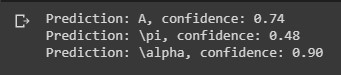
\includegraphics[width=4cm]{figures/1174066/7/no20.jpg}
	\caption{Hasil No 20}
\end{figure}
\subsection{Penanganan Error}
\subsubsection{Error}
\hfill\break
\begin{itemize}
\item ProfilerNotRunningError

\begin{figure}[H]
\centering
	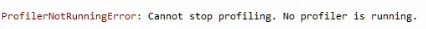
\includegraphics[width=4cm]{figures/1174066/7/error1.jpg}
\caption{ProfilerNotRunningError}
\end{figure}
\end{itemize}
\subsubsection{Solusi Error}
\hfill\break
\begin{itemize}
\item ProfilerNotRunningError

tambahkan kode profile=10000000 pada parameter log\_dir
\end{itemize}

\subsection{Bukti Tidak Plagiat}
\begin{figure}[H]
	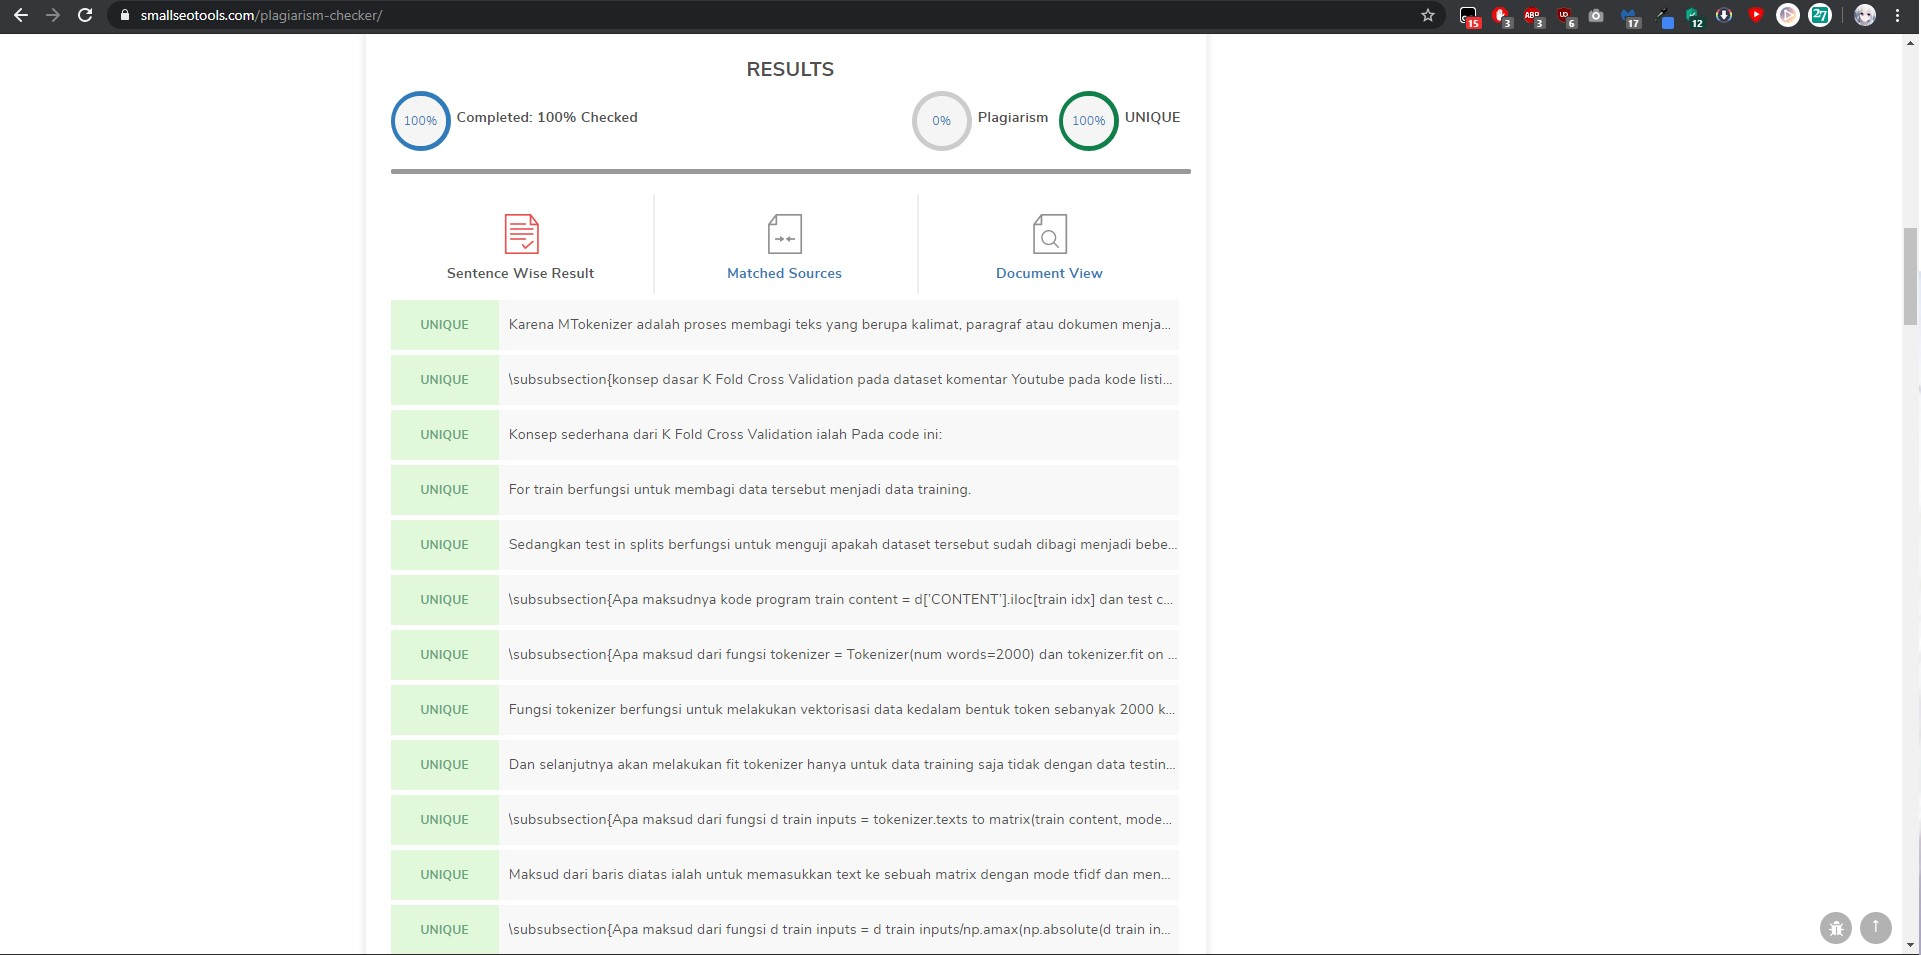
\includegraphics[width=4cm]{figures/1174066/7/buktiplagiat.jpg}
	\centering
	\caption{Bukti tidak plagiat}
\end{figure}

\subsection{Link Youtube}
https://youtu.be/Vq\_LZ89hTpg